% Template for ICASSP-2016 paper; to be used with:
%          spconf.sty  - ICASSP/ICIP LaTeX style file, and
%          IEEEbib.bst - IEEE bibliography style file.
% --------------------------------------------------------------------------
\documentclass{article}
\usepackage{spconf,amsmath,graphicx}
\usepackage{natbib}

% Example definitions.
% --------------------
\def\x{{\mathbf x}}
\def\L{{\cal L}}

% Title.
% ------
\title{Training Recurrent Neural Networks with Batch Normalization}

\name{C\'{e}sar Laurent$^\ast$, Gabriel Pereyra$^\dagger$, Phil\'{e}mon
Brakel$^\ast$, Ying Zhang$^\ast$ and
Yoshua Bengio$^\ast{}^1$}
\address{
  $^\ast$ Universit\'e de Montr\'eal\\
  $^\dagger$University of Southern California\\
  ${^1}$ CIFAR Fellow}
%
% Single address.
% ---------------
%\name{Author(s) Name(s)\thanks{Thanks to XYZ agency for funding.}}
%\address{Author Affiliation(s)}
%
% For example:
% ------------
%\address{School\\
%	Department\\
%	Address}
%
% Two addresses (uncomment and modify for two-address case).
% ----------------------------------------------------------
%\twoauthors
%  {A. Author-one, B. Author-two\sthanks{Thanks to XYZ agency for funding.}}
%	{School A-B\\
%	Department A-B\\
%	Address A-B}
%  {C. Author-three, D. Author-four\sthanks{The fourth author performed the work
%	while at ...}}
%	{School C-D\\
%	Department C-D\\
%	Address C-D}
%
\begin{document}
%\ninept
%
\maketitle
%
\begin{abstract}
Training Recurrent Neural Networks (RNNs) is often times prohibitively expensive, particularly 
for deep architectures. Batch normalization, a method for normalizing intermediate 
representations of neural networks using batch statistics, has proven to significantly reduce 
training times of very deep convolutional neural networks. Here, we show how to apply batch
normalization to RNNs, which leads to faster convergence.

\end{abstract}
%
\begin{keywords}
batch normalization, RNN, optimization, speech recognition, language model
\end{keywords}
%
\section{Introduction}

Recurrent Neural Networks (RNNs) have received renewed interest due to their recent successes across a number of domains. In speech recognition, RNNs are able to learn mappings from speech to text, matching state of the art without the need for an alignment model [?]. In machine translation, encoder-decoder, or sequence-to-sequence models, are able map arbitrary length sequences of one language to another, learning the alignment on the fly. For language models, RNNs have recent been shown to learn expressive semantic embeddings and the ability to model long term grammatical dependencies, such as opening and closing parenthesis [?].

Despite the expressiveness of these models, the training cost for large datasets and deep architectures of stacked RNNs can be prohibitively expensive, often times an order of magnitude greater than other models [?]. Because of this, recent work has explored methods for parallelizing RNNs across multiple GPUs. In [?], a RNN was distributed layer wise across 8 GPUs, with the softmax taking half of the GPUs. Similarly, in [?], a RNN was distributed across time, with the forward and backward pass of a Bi-Directional RNN layer being split in half. However, due to the sequential nature of RNNs, the speedups of multiple GPUs is far from linear.

Another way to reduce training times is through a better conditioned optimization. Standardizing or whitening of input data has long been known to improve convergence of optimization methods [?]. Extending this idea to multi-layered networks suggests that normalizing or whitening intermediate representations can similarly improve convergence. However, naively applying these transforms would be extremely costly. In [?], batch normalization was used to standardize intermediate representations by approximating the population statistics with the min-batch. Similarly, in [?], showed that by minimizing the natural gradient and calculating ?, one can go one step further and whiten intermediate representations.

These methods reduced training times of Convolutional Neural Networks (CNNs) by an order of magnitude and additionallly provided a regularization constraint. In this paper, we explore how to leverage normalization in RNNs and show that training time can be significantly reduced.

\section{Batch Normalization}

In optimization, standardization or whitening is a common procedure proven to reduce asymptotic convergence rates. By better conditioning the optimization procedure, algorithms like gradient descent are able to take better steps in the direction of the minimum. Extending the idea to deep neural networks, one can think of an arbitrary layer as receiving an input distribution from the previous layer. Normally, this distribution changes every update, making layer responsible, not only for learning a good representation but for adapting to a changing distribution as well. The changing distribution of the intermediate distributions of a network is termed covariate drift and reducing this drift is hypothesized to be the reason why batch normalization significantly reduces training times.

Since, calculating population statistics over a large dataset after every update is infeasible, batch normalization approximates them with sample statistics drawn from a mini-batch. Given a batch of samples $\x_1, \dots \x_n$, we can calculate the sample mean and sample standard deviation as

\begin{equation}
	\begin{split}
		& \bar \x = \frac{1}{n} \sum_i^n \x_i \\
		& \boldsymbol{\sigma} = \frac{1}{n} = \sum (\x_i - \hat \x)
	\end{split}
\end{equation}

and using these statistics, we can standardize the data as follows

\begin{equation}
	\hat \x = \frac{\x - \bar \x}{\boldsymbol \sigma}
\end{equation}

However, by simply standardizing the intermediate representation, the representational power of the layer is changed. To account for this, batch normalization introduces additional learnable parameters $\gamma$ and $\beta$, which respectively scale and shift the data, leading to a layer of the form

\begin{equation}
	BN(x) = \gamma \hat \x + \beta
\end{equation}

By setting $\gamma$ to the standard deviation and $\beta$ to the expectation, we can recover the original layer representation.

At test time, we can calculate mean and sigma in a number of ways. The simplest is to use a validation batch as was done during training. Alternatively, population statistics can be calculated at the end of training or during training by maintaining a running average calculated over each mini-batch seen during training.

\section{Recurrent Neural Networks}
RNNs maintain a hidden vector $\boldsymbol h$, which is updated at time step $t$ as follows:
 
\begin{equation}
	\boldsymbol h_t = \tanh(\boldsymbol W * \boldsymbol h_{t-1} + \boldsymbol I * \x_t) \nonumber
\end{equation}

Where $\tanh$ is the hyperbolic tangent function, $\boldsymbol W$ is the recurrent weight matrix and $I$ is a projection matrix. The hidden state $\boldsymbol h$ is then used at each time step in the case of language modeling or at the end of the sequence to make a prediction $\boldsymbol y$

\begin{equation}
	\boldsymbol y_t = softmax(\boldsymbol W * \boldsymbol h_{t-1}) \nonumber
\end{equation}

where $softmax$ provides a normalized probability distribution over the possible classes and $\boldsymbol W$ is a weight matrix. By using $\boldsymbol h$ as the input to another RNN, we can stack RNNs, creating deeper architectures [?]

\begin{equation}
	\boldsymbol h_t^{l} = \sigma(\boldsymbol W * \boldsymbol h_{t-1}^{l} + \boldsymbol I * \boldsymbol h_t^{l-1}) \nonumber
\end{equation}

Training vanilla RNNs is known to be particularly difficult, primarily due to the vanishing gradient problem [?].

\subsection{Long Short-Term Memory}
LSTMs address the vanishing gradient problem commonly found in RNNs by incorporating gating functions into their state dynamics [?]. At each time step, an LSTM maintains a hidden vector $\boldsymbol h$ and a memory vector $\boldsymbol m$  responsible for controlling state updates and outputs. More concretely, we define the computation at time step $t$ as follows [?]:

\begin{equation}
	\begin{split}
		& \boldsymbol g^u = \sigma(\boldsymbol W^u * \boldsymbol h_{t-1} + \boldsymbol I^u * \x_t) \\
		& \boldsymbol g^f = \sigma(\boldsymbol W^f * \boldsymbol h_{t-1} + \boldsymbol I^f * \x_t) \\
		& \boldsymbol g^o = \sigma(\boldsymbol W^o * \boldsymbol h_{t-1} + \boldsymbol I^o * \x_t) \\
		& \boldsymbol g^c = \tanh(\boldsymbol W^c * \boldsymbol h_{t-1} + \boldsymbol I^c * \x_t) \\
		& \boldsymbol m_t = \boldsymbol g^f \odot \boldsymbol +  \boldsymbol g^u \odot \boldsymbol g^c \\
		& \boldsymbol h_t = \tanh(\boldsymbol g^o \odot \boldsymbol m_{t-1}) \nonumber
	\end{split}
\end{equation}

Where $\sigma$ is the logistic sigmoid function, $\boldsymbol W^u, \boldsymbol W^f, \boldsymbol W^o, \boldsymbol W^c$ are recurrent weight matrices and $\boldsymbol I^u, \boldsymbol I^f, \boldsymbol I^o, \boldsymbol I^c$ is are projection matrices.

\section{Normalization}

The more complicated state transition of LSTMs as compared to CNNs allows for a number of batch normalized variants. With respect to batch normalization, we applied the normalization procedure in a number of different locations in the LSTM equations.

\subsection{Projection Normalization} The simplest method for normalizing LSTMs is applying batch normalization only on the input to hidden transition, as these are independent of previous hidden states. Generalizing the gate equations given above, we can express this form as

\begin{equation}
	\boldsymbol g = \sigma(\boldsymbol W * \boldsymbol h + BN(\boldsymbol I * \x)) \\
\end{equation}
 
Where batch normalization is applied after the input projection $\boldsymbol I$ and then summed with the new hidden state $\boldsymbol h$ before applying the gate non-linearity.

\subsection{State Normalization} Similarly, we can normalize only the the hidden state transitions by applying batch normalization after applying the recurrent weight matrix $\boldsymbol W$ to the previous hidden state $\boldsymbol h_{t-1}$

\begin{equation}
	\boldsymbol g = \sigma(BN(\boldsymbol W * \boldsymbol h_{t-1}) + \boldsymbol I * \x) \\
\end{equation} 

\subsection{Gate Normalization} Combining the two methods above, we can normalize all the gates, leading to 

\begin{equation}
	\boldsymbol g = \sigma(BN(\boldsymbol W * \boldsymbol h + \boldsymbol I * \x)) \nonumber
\end{equation}

\subsection{Temporal Normalization}
We can extend batch normalization to sequences by calculating a reduction across steps in the sequence instead of along the batches (or in addition to). Given a sequence of length $t$, we normalize across the sequence as follows

\begin{equation}
	\begin{split}
		& \hat \x_t = \frac{\boldsymbol x - \frac{1}{t} \sum \x_t}{\sqrt{Var(\x_t)}} \\
		& TN(\x) = \gamma \hat \x_t + \beta
	\end{split}
\end{equation}

As a note of caution, one must take care not to normalize across the time information in tasks where this leads to using future statistics to make past predictions. For example, RNN language models usually predict the next token at each time step. If time normalization is used in this case, the model learns to use future time steps to make predictions about the next token, which equates to using labeled data to make predictions.

\subsection{Adaptive Learning Rates} One challenge of normalizing RNNs is that by normalizing individual components, we change the learning dynamics of that component in relation to the others. In their experiments, [?] noted that batch normalization allows for much higher learning rates. However, in the case where we normalized the input projection and optimize with stochastic gradient descent, a higher learning rate leads to vanishing gradients because negatively effects the recurrent weight updates. To address this, we can use a different learning rate for these transition or employ an optimizer with adaptive learning rates, such as RMSprop.


\section{Experiments}

\subsection{Language Modeling}
We used the Penn Treebank (PTB) [?] corpus for our language modeling experiments. We use the standard split (929k training words, 73k validation words, and 82k test words) and vocabulary of 10k words. We train a small LSTM and a Large LSTM as described in [?].

Both models consist of two stacked LSTM layers and are trained with stochastic gradient descent with a learning rate of 1 and a mini-batch size of 20.

The small LSTM has a hidden size of 200 for both layers, initialized uniformly in the range [-0.1, 0.1]. We back propagate across 20 time steps and gradients are scaled according to the maximum norm of the gradients whenever the norm is greater than 10 [?]. We train for 15 epochs and halve the learning rate every epoch after the 6th.  

The Large LSTM has a hidden size of 1500 for both layers, initialized uniformly in the range [-0.04, 0.04]. We apply dropout between all layers. We back propagate across 35 time steps and gradients are scaled according to the maximum norm of the gradients whenever the norm is greater than 5 [?]. We train for 55 epochs and divide the learning rate by 1.15 every epoch after the 15th.

\begin{figure}[t]
  \centering
  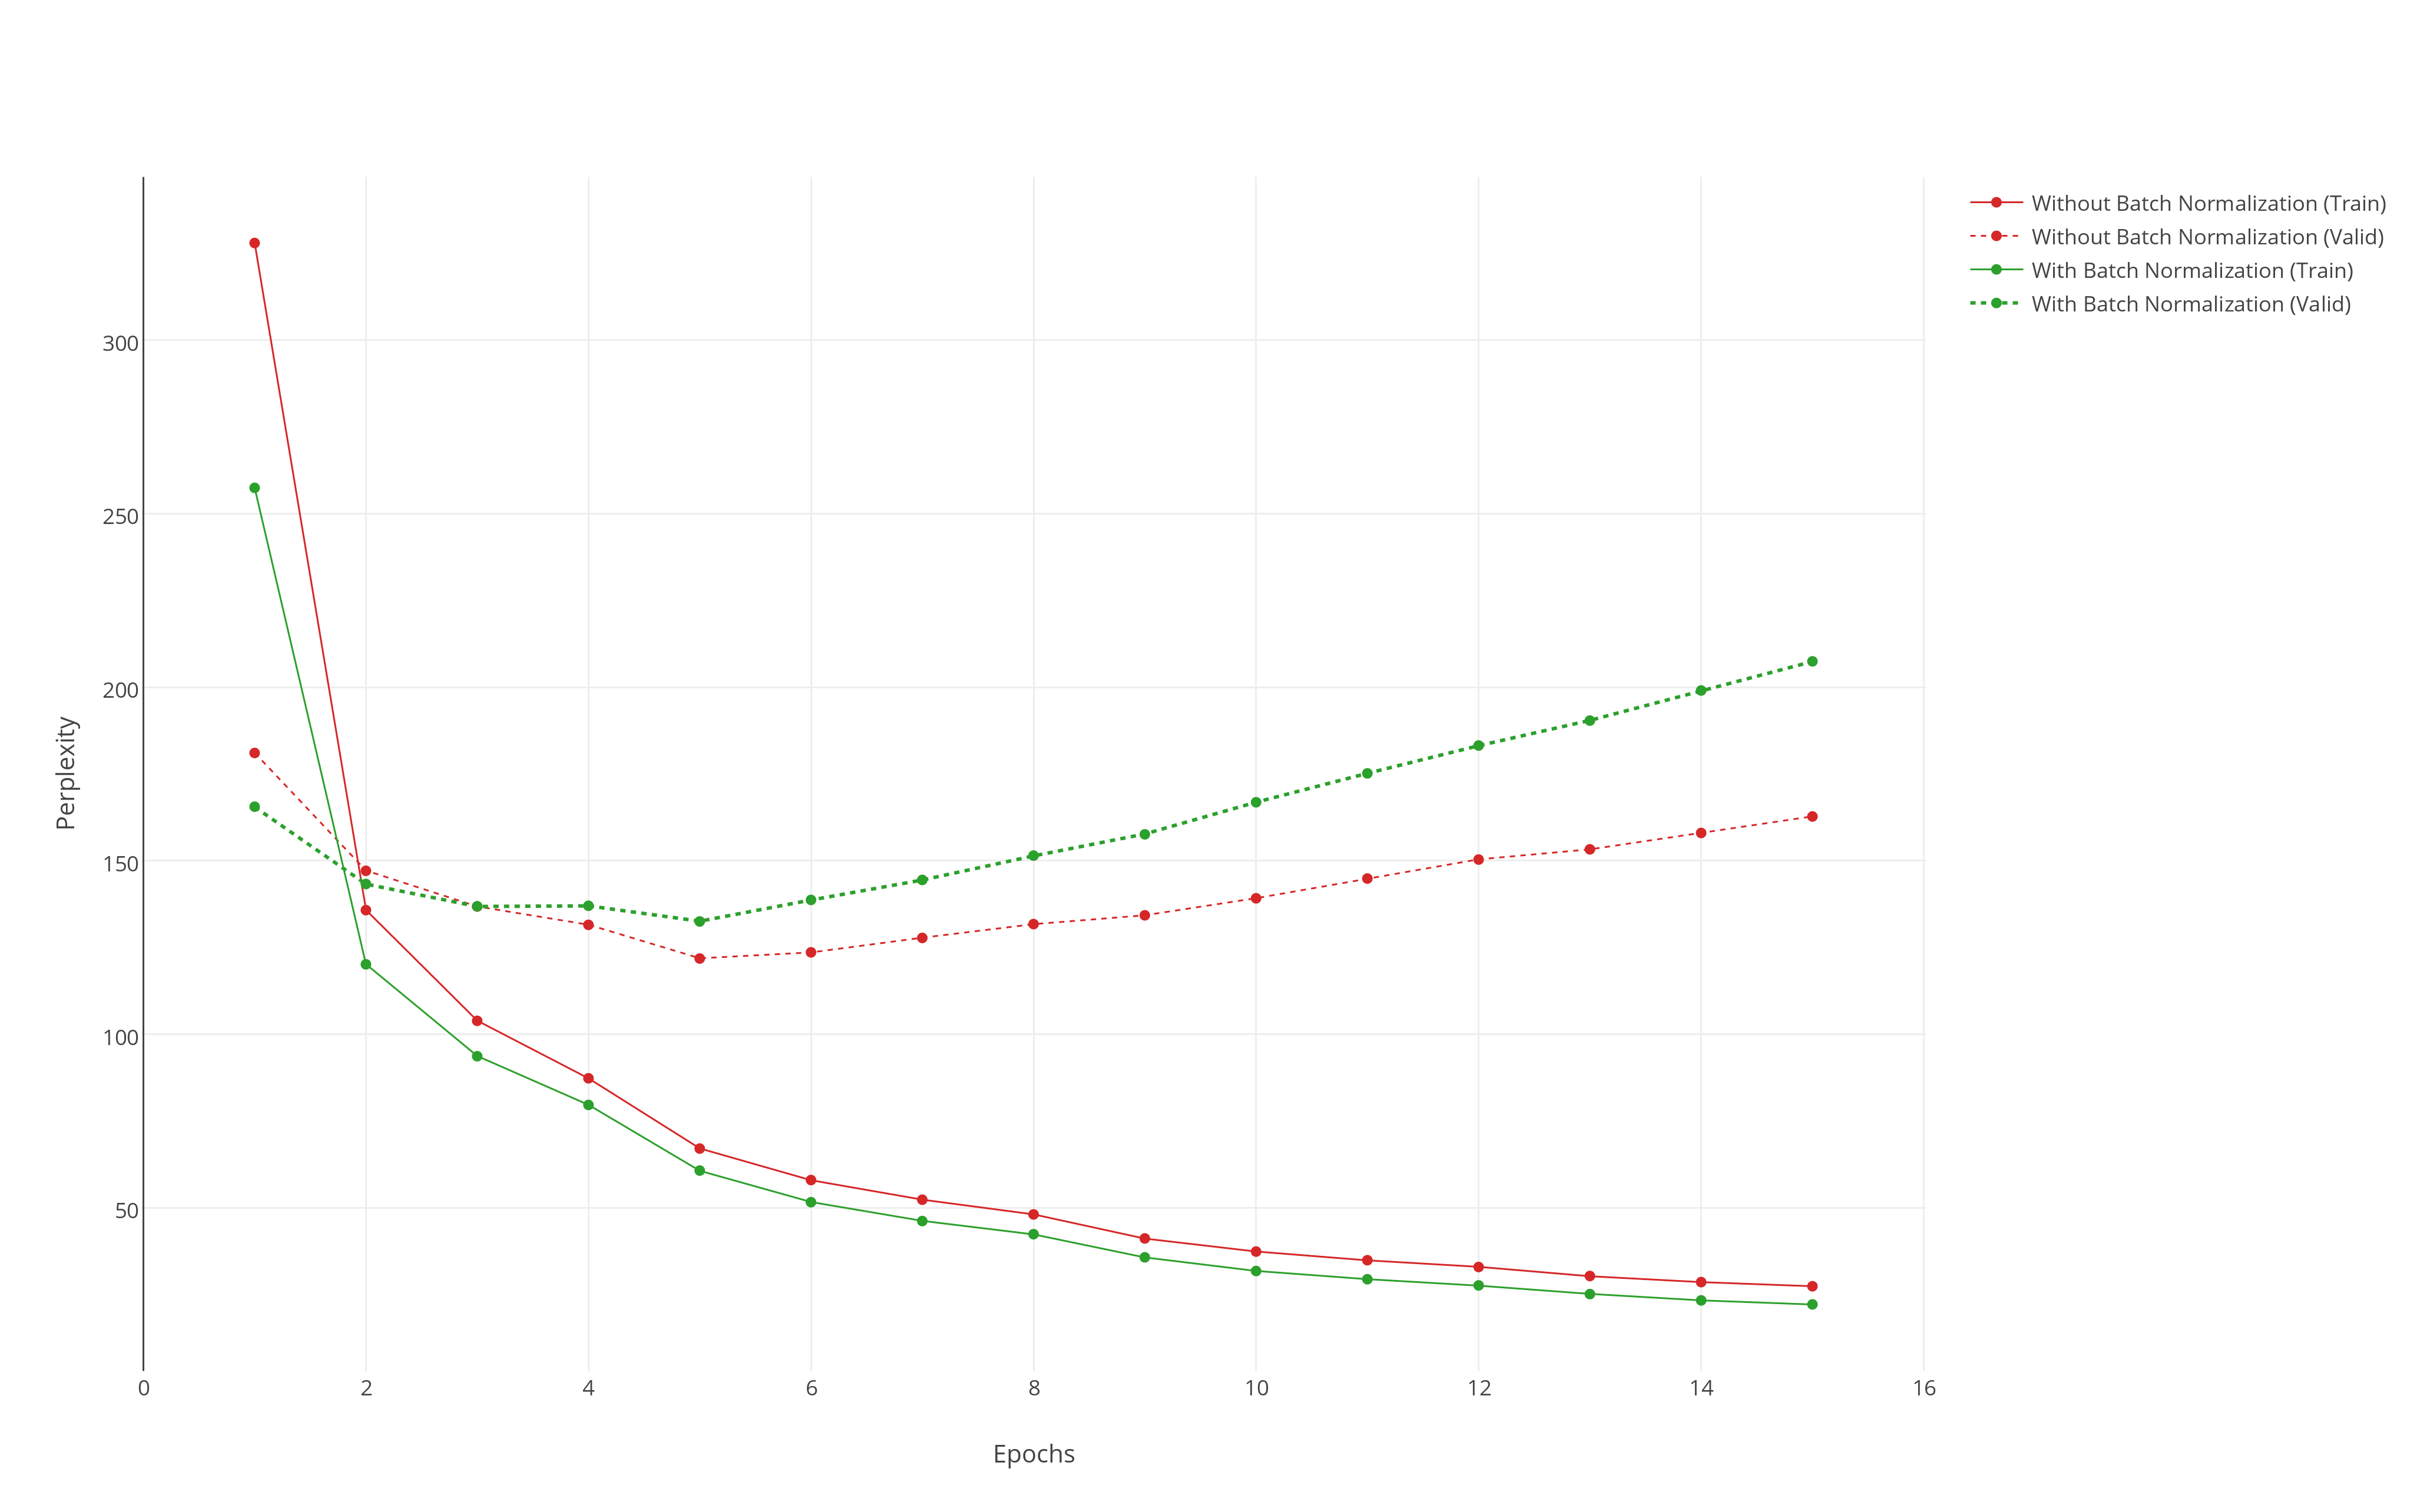
\includegraphics[width=100mm]{ptb_small_norm_plot.png}
  \caption{[Plot iterations instead of epochs, move legend to bottom and make font/lines larger] Small LSTM on Penn Treebank with and without batch normalization.}
  \label{overflow}
\end{figure}


{\renewcommand{\arraystretch}{1.4}

\begin{table}
	\begin{center}
		\begin{tabular}{lcr}
  			\hline
  			
			\multicolumn{1}{l}{\bf Model}  &\multicolumn{1}{c}{\bf Valid Set}  &\multicolumn{1}{c}{\bf Test Set} \\
  			
			\hline
  			
			\multicolumn{3}{c}{Penn Treebank} \\
  			
			\hline

  			Small LSTM		& 120.7 & 114.5 \\
  			Small LSTM (BN)	& 130.0 & 123.9 \\

  			\hline

  			Large LSTM		& 82.2 & \textbf{78.4} \\
  			Large LSTM (BN)	& \\

  			\hline

		\end{tabular}
	
		\caption{[\textit{Bold top and bottom lines}] Word-level perplexity on the Penn Treebank dataset.}

	\end{center}
\end{table}

\subsection{Speech Recognition}

\section{Discussion}

% References should be produced using the bibtex program from suitable
% BiBTeX files (here: strings, refs, manuals). The IEEEbib.bst bibliography
% style file from IEEE produces unsorted bibliography list.
% -------------------------------------------------------------------------
%\bibliographystyle{IEEEbib}

\bibliographystyle{natbib}
\bibliography{paperrefs}

\end{document}
